\subsubsection{\textbf{Graph Vector Edit Distance (GVED)}} 
Structure-oriented approaches in code semantic comparision have become popular in programming. In many popular tructure-orientedd approaches nowadays, Exas is an accurate and efficient structural characteristic feature extraction approach that better approximates and captures the structure within the fragments of artifacts.\cite{Accurate and Efficient Structural Characteristic Feature Extraction for Clone Detection}.
In our study area, we use Exas as a mean of computing the difference between code structure. Given a pair of method in C\# which are need to be compared their structure, GROUM [cite GROUM] is used to parse code into program dependence graphs (PDGs) [cite to PDG] and Exas continues processing these graphs. In Exas, the characteristic features are extracted from the patterns of elements of the graphs. The code fragments are characterized by their counting vectors of those features. The difference between two vectors reflects the difference of two graphs.  Therefore, distance of these counting vectors is considered the way to measure the sematic between code fragments.



Figure \ref{fig:PDGs} shows an illustrated PGDs of a code fragment 1 and fragment 2 which are parsed by GROUM. These graphs are analysed by Exas, which focuses on two kinds of patterns of structural information of the graph, called (p, q)-node and n-path as can be seen at table \ref{tab:feature1} and table \ref{tab:feature2}. 

An efficient way to express the property ``having the same or similar features`` is the use of vectors. The characteristic vector of a fragment is the occurrence-count vector of its features. That is, each position in the vector is indexed for a feature and the value at that position is the number of occurrences of that feature in the fragment. Table \ref{tab:featureIndex} shows the indexes of the features, which are global across all vectors. Based on the occurrence counts this table, the vectors for code1 and code2 are V1(1,1,1,1,1,0,1,0...),V2(1,1,0,1,1,1,1,1...) respectively. Two fragments having the same feature sets and occurrence counts will have the same vectors and vice versa. The vector similarity can be measured by an appreciably chosen vector distance such as 1-norm distance.


\begin{lstlisting}[language=JAVA]
	Code 1:
	void foo(int i) {
		int j;
		if (i < 2) {
			j = 1;
		} else {
			j = 2;
		}
	}

	Code 2:
	void foo(int i) {
		int j;
		if (i < 2) 
			j = i;	 
		j = 2;
	}
\end{lstlisting}
\begin{figure}[h]
	\caption{An example: two PDGs represent code1 and code2}
	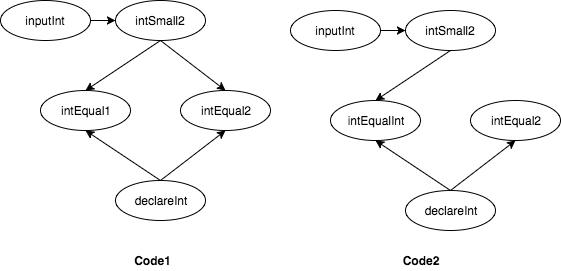
\includegraphics[scale=0.4]{img/Diagram_PDG.png}
	\centering
	\label{fig:PDGs}
\end{figure}

% Table generated by Excel2LaTeX from sheet 'Sheet1'
\begin{table}[htbp]
  \centering
  \caption{Feature table of code1 extracted in Exas}
  \scalebox{0.65}{
    \begin{tabular}{|l|l|l|l|l|r|}
    \toprule
    \textbf{Pattern} & \multicolumn{5}{c|}{\textbf{Feature of Code1}} \\
    \midrule
    \textit{\textbf{1-path}} & inputInt & intSmall2 & intEqual1 & intEqual2 & \multicolumn{1}{l|}{declareInt} \\
    \midrule
    \textit{\textbf{2-path}} & \multicolumn{1}{p{6.415em}|}{inputInt-intSmall2} & \multicolumn{1}{p{5.915em}|}{intSmall2-intEqual1} & \multicolumn{1}{p{6em}|}{intSmall2-intEqual2} & \multicolumn{1}{p{5.75em}|}{declareInt-intEqual1} & \multicolumn{1}{p{5em}|}{declareInt-intEqual2} \\
    \midrule
    \textit{\textbf{3-path}} & \multicolumn{1}{p{6.415em}|}{intputInt-intSmall2-intEqual1} & \multicolumn{1}{p{5.915em}|}{intputInt-intSmall2-intEqual2} &       &       &  \\
    \midrule
    \textit{\textbf{(p,q)-node}} & inputInt-0-1 & intSmall2-1-2 & intEqual1-2-0 & intEqual2-1-2 &  \\
    \bottomrule
    \end{tabular}%
	}
  \label{tab:feature1}%
\end{table}%

% Table generated by Excel2LaTeX from sheet 'Sheet1'
\begin{table}[htbp]
  \centering
	\caption{Feature table of code2 extracted in Exas}
	\scalebox{0.65}{
	    \begin{tabular}{|l|l|l|l|l|r|}
    \toprule
    \textbf{Pattern} & \multicolumn{5}{c|}{\textbf{Feature of Code2}} \\
    \midrule
    \textit{\textbf{1-path}} & inputInt & intSmall2 & intEqualInt & intEqual2 & \multicolumn{1}{l|}{declareInt} \\
    \midrule
    \textit{\textbf{2-path}} & \multicolumn{1}{p{6.415em}|}{inputInt-intSmall2} & \multicolumn{1}{p{5.915em}|}{intSmall2-intEqualInt} & \multicolumn{1}{p{6em}|}{declareInt-intEqual1} & \multicolumn{1}{p{5.75em}|}{declareInt-intEqual2} &  \\
    \midrule
    \textit{\textbf{3-path}} & \multicolumn{1}{p{6.415em}|}{intputInt-intSmall2-intEqualInt} &       &       &       &  \\
    \midrule
    \textit{\textbf{(p,q)-node}} & inputInt-0-1 & intSmall2-1-1 & intEqualInt-2-0 & intEqual2-1-0 &  \\
    \bottomrule
    \end{tabular}%
	}
  \label{tab:feature2}%
\end{table}%

% Table generated by Excel2LaTeX from sheet 'Sheet1'
\begin{table}[htbp]
	\centering
	\caption{Feature Indexing}
	\scalebox{0.75}{
	\begin{tabular}{|cccc|}
		\toprule
		\multicolumn{1}{|l|}{\textbf{Feature}} & \multicolumn{1}{l|}{\textbf{Index}} & \multicolumn{1}{l|}{\textbf{Counted in Code1}} & \multicolumn{1}{l|}{\textbf{Counted in Code2}} \\
		\midrule
		\multicolumn{1}{|l|}{inputInt} & \multicolumn{1}{r|}{1} & \multicolumn{1}{r|}{1} & \multicolumn{1}{r|}{1} \\
		\midrule
		\multicolumn{1}{|l|}{intSmall2} & \multicolumn{1}{r|}{2} & \multicolumn{1}{r|}{1} & \multicolumn{1}{r|}{1} \\
		\midrule
		\multicolumn{1}{|l|}{intEqual1} & \multicolumn{1}{r|}{3} & \multicolumn{1}{r|}{1} & \multicolumn{1}{r|}{0} \\
		\midrule
		\multicolumn{1}{|l|}{intEqual2} & \multicolumn{1}{r|}{4} & \multicolumn{1}{r|}{1} & \multicolumn{1}{r|}{1} \\
		\midrule
		\multicolumn{1}{|l|}{declareInt} & \multicolumn{1}{r|}{5} & \multicolumn{1}{r|}{1} & \multicolumn{1}{r|}{1} \\
		\midrule
		\multicolumn{1}{|l|}{intEqualInt} & \multicolumn{1}{r|}{6} & \multicolumn{1}{r|}{0} & \multicolumn{1}{r|}{1} \\
		\midrule
		\multicolumn{1}{|p{5.75em}|}{inputInt-intSmall2} & \multicolumn{1}{r|}{7} & \multicolumn{1}{r|}{1} & \multicolumn{1}{r|}{1} \\
		\midrule
		\multicolumn{1}{|l|}{intEqual2-1-0} & \multicolumn{1}{r|}{8} & \multicolumn{1}{r|}{0} & \multicolumn{1}{r|}{1} \\
		\midrule
		\multicolumn{4}{|c|}{To be continued} \\
		\bottomrule
	\end{tabular}%
	}
	\label{tab:featureIndex}%
\end{table}%


We introduce the formuala for normalizing the result of vector edit distance which is used in the next part of the paper. The normalized value is described as

$GVED(V1, V2) = 1 - \sum_{i=1}^{n} \frac{ \mid XV1_i - XV2_i \mid}{XV1_i + XV2_i}$, 
where $n$ denotes the number of vector scalar, $V1$ denotes the counting vector of the first graph, $V2$ denotes the counting vector of the second graph, $XV1_i$ denotes $V1$\rq the value of the $i-th$ scalar, $XV2_i$ denotes $V2$\rq the value of the $i-th$ scalar.  

In this example, the value of GVED is $GVED(V1, V2) = 1 - \frac{8 }{20} = 0.6$.
